%\documentclass{article}
\documentclass[aps,prl,amssymb,amsmath,twocolumn,floatfix]{revtex4}
\usepackage{graphicx}
\usepackage{amsmath}



\newcommand{\vx}{\mathbf{x}}
\newcommand{\vy}{\mathbf{y}}

\begin{document}
\title{Blume-Cappel model analysis with Rose-Machta micro-canonical annealing method}
\author{Vyacheslav Mozolenko$^{1,2}$}
\author{Lev Shchur$^{1, 2}$}
\affiliation{$^1$ HSE University, 101000 Moscow, Russia}
\affiliation{$^2$ Landau Institute for Theoretical Physics, 142432 Chernogolovka, Russia}


\begin{abstract}
We analyze critical behavior of Blume-Capel model using the micro-canonical annealing method introduced recently by Rose and Machta (PRE, 100 (2019) 063304). We use cooling-heating modification of the Rose-Machta method, and estimate entropy of the model and calculate energy and specific heat, from which we estimate critical temperature. The results are in a good agreement with the known values estimated using various methods -- conventional Monte Carlo methods, Wang-Landau method, and series expansions. We found the Rose-Machta method for estimation of the density of states is faster and allows using larger lattice sizes in comparison with the Wang-Landau method.

\end{abstract}

\maketitle

\section{Introduction}


Second order phase transition - Critical slowing down (CSD)

First order phase transition - Exponential critical slowing down (ECSD), time scale for the simulation growth with $L$ as $\exp\left(\sum L^{D-1}\right)$, where $L$ is the system size, $D$ - system dimension, and $\sum$ is the surface tension of the interface build between phases~\cite{VMM-2007}


\section{Micro-canonical annealing - EMA}

In this section we present main ideas of the Rose-Machta method for the direct estimation of the density of states and our modification of the method, in which we use cooling and heating of the samples generated with random configuration. 

\subsection{Rose-Machta EMA method}

In article \cite{Machta} John Machta and Natan Rose introduced new technique for modeling system's microcannonicle ensemble by using annealing under energy ceiling. By design, this technique is meant for obtaining numerical values of density of states, (DOS, g(E)). 

Algorithm read as follows:
Let us assume R replica of our system, for example, Potts-3 spin system, for which we know or minimal spectrum step, or the spectrum itself. (Inside of each replica we fill spins consequentially with randomly chose spin, by using default RNG for GNU SL - MT19937.)

0. Let us define upper energy ceiling $U > E_{max}$. On each step:

1. We allow replica to thermalize during some predefined time $T$ with acceptance of all spin switches, if only it does not raise replica energy above ceiling $U$. (one can call it an infinite temperature thermalization). Choosing of a spin and of new spin value we perform by default RNG for CUDA - XORWOW.

2. Let us lower $U$ by one minimal spectrum step (or onto the next energy in the spectrum); filter $R^*$ replica with $E_i = U$ and write down its ratio $\epsilon(U) = R^*/R$.

3. Rest $R-R^*$ replica, which were under the new ceiling $U$, we propagate randomly to fill the previous number of replica $R$


\begin{figure}[h!]
	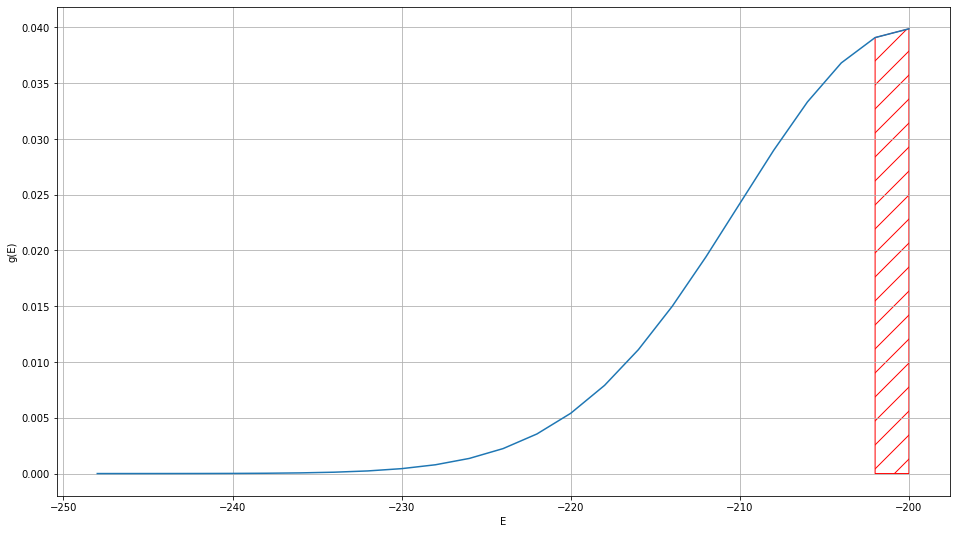
\includegraphics[width=\linewidth]{DOS_slice_picture.png}
	\caption{An example of how density of states behaves on every step. Hatched area - the $\epsilon(E)$ replica, which we filter on current step; $N=400$}
\end{figure}


This cycle we continue until $U=E_{min}$. AS we know $\epsilon(U)$ and ground state (GS) multiplicity we can restore the density of states from GS up by energy spectrum (see \postcalc).

Let us note the problems, associated with this algorithm. As far as replicas exist in "effective infinite temperature",  the number of replicas on edges of the spectrum will be exponentially low; thus, if we "cool" out system, we will not get any information on high-energy part of the spectrum: $\epsilon(E)$ will be close to 0 until we first reach energies E, occupied with replicas (near entropy maximum).

The other problem is rather technical, yet rather annoying. For the algorithm we need to know the energy spectrum (or minimum spectrum step), which is not always possible or practical.


\subsection{Our cooling-heating modification with adaptive step of Rose-Machta method}

\subsection{Cooling}

Let us assume R replica of our system. (Inside of each replica we fill spins consequentially with randomly chose spin, by using in-build RNG for CUDA SL - $Philox_4x32_10$.)

0. Let us define upper energy ceiling $U > E_{max}$. On each step:

1. We allow replica to thermalize during some predefined time $T$ with acceptance of all spin switches, if only it does not raise replica energy above ceiling $U$. (one can call it an infinite temperature thermalization). Choosing of a spin and of new spin value we perform by in-build RNG for CUDA SL - $Philox_4x32_10$.

2.1. For each replica we calculate its current energy and find the maximum among them (Obvious, $E_{max} < U$);

2.2. Let us lower $U$ to newfound maximum energy $E_{max}$; filter $R^*$ replica with $E_i = U$ and write down its ratio $\epsilon(U) = R^*/R$.

3. Rest $R-R^*$ replica, which were under the new ceiling $U$, we propagate randomly to fill the previous number of replica $R$

This cycle we continue until on one step we filter all our replica.


\subsection{Heating}

To obtain upper part of our energy spectrum, we need to "invert" our algorithm and instead of cooling and lowering energy ceiling $U$, we need to heat and raise energy floor (to confuse the reader, we named it $U$ as well). 

Let us assume R replica of our system. (Inside of each replica we fill spins consequentially with randomly chose spin, by using in-build RNG for CUDA SL - $Philox_4x32_10$.)

0. Let us define lower energy floor $U > E_{max}$. On each step:

1. We allow replica to thermalize during some predefined time $T$ with acceptance of all spin switches, if only it does not raise replica energy below floor $U$. (one can call it an infinite temperature thermalization). Choosing of a spin and of new spin value we perform by in-build RNG for CUDA SL - $Philox_4x32_10$.

2.1. For each replica we calculate its current energy and find the minimum among them (Obvious, $E_{min} > U$);

2.2. Let us raise $U$ to newfound minimum energy $E_{min}$; filter $R^*$ replica with $E_i = U$ and write down its ratio $\epsilon(U) = R^*/R$.

3. Rest $R-R^*$ replica, which were under the new ceiling $U$, we propagate randomly to fill the previous number of replica $R$

This cycle we continue until on one step we filter all our replica.

\subsection{Postcalculation of $\epsilon(E)$ into $S(E)$}
For cooling or original algorithm:
$$
S(E) = \ln(\epsilon(E)) + \sum_{E'>E} \ln(1 - \epsilon(E'))
$$
For heating: 
$$
S(E) = \ln(\epsilon(E)) + \sum_{E'<E} \ln(1 - \epsilon(E'))
$$

After we obtained both "halves" of $S(E)$, we "stitch" them by intersecting part (more precisely, along the central third of the part common to them).


\subsection{Potts example}
{\bf VM - please, describe in details the cooling-heating method from random configuration. Please, provide shortly details of your results for the Potts model.}

\section{Blume-Capel model}

\section{Simulations}

\begin{figure}
  \centering
  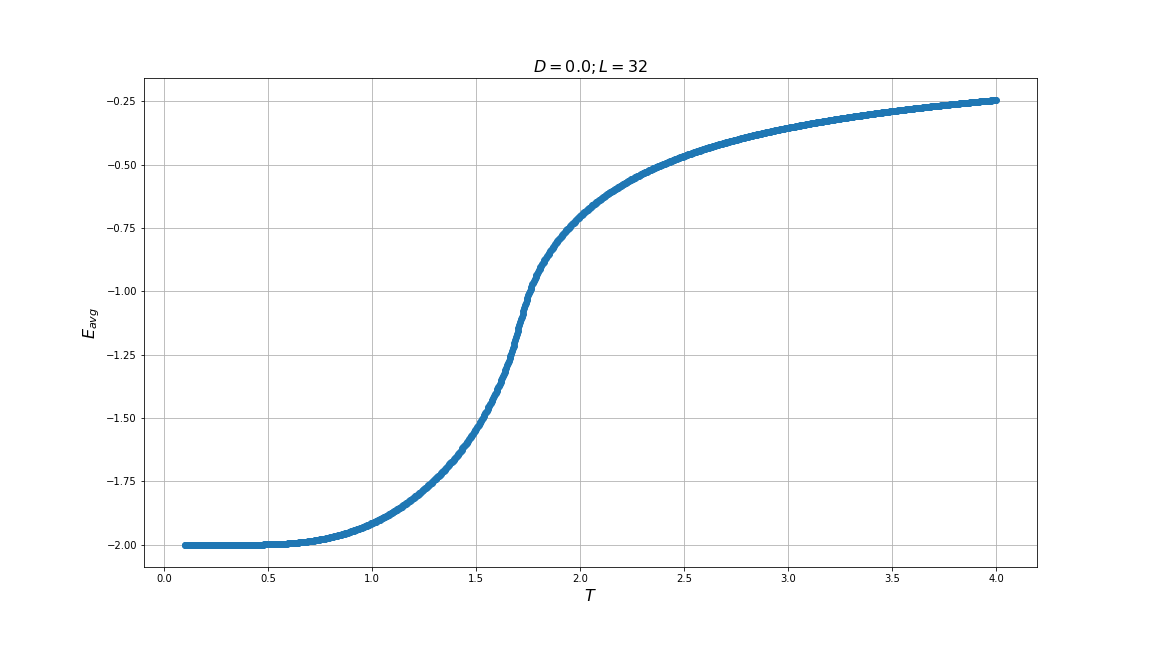
\includegraphics[width=.95\linewidth]{E_avg(T)_D0.0_L32.png}
  \caption{Energy of Blume-Cappel model. D/J=0.}
  \label{fig:BC-E-0}
\end{figure}
\begin{figure}
  \centering
  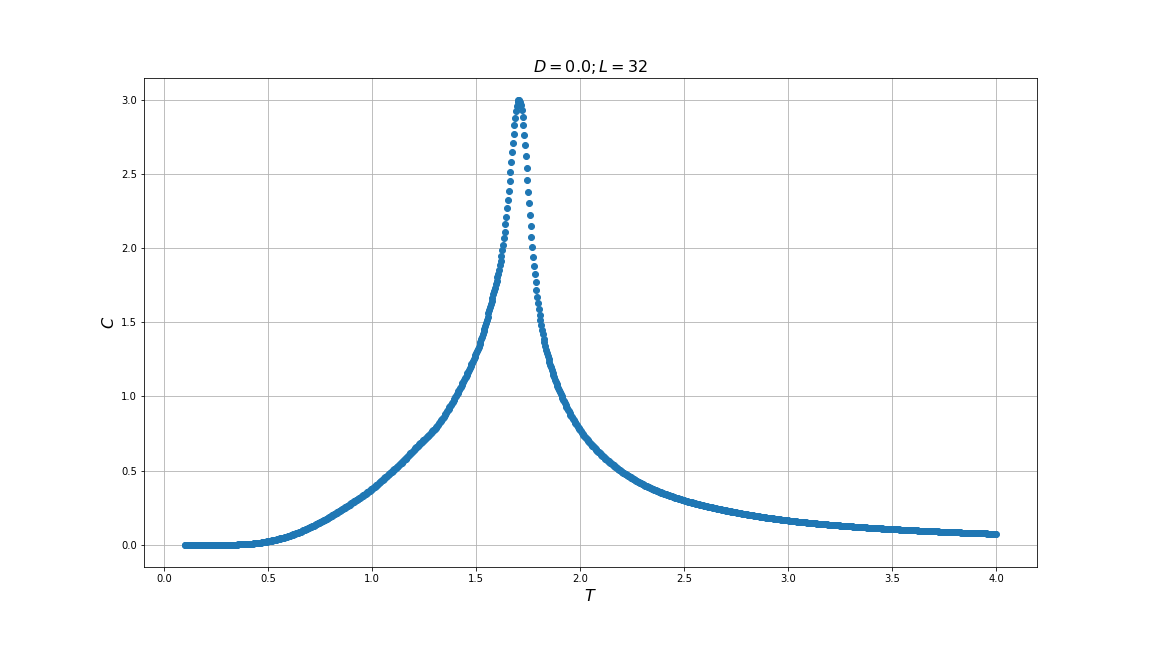
\includegraphics[width=.95\linewidth]{C(T)_D0.0_L32.png}
  \caption{Specific heat of Blume-Cappel model. D/J=0. }
  \label{fig:BC-C-0}
\end{figure}


\section{Data analysis}

\subsection{Estimation of critical temperature and critical behaviour}

The two major terms in the finite-size dependence of the specific heat of Ising model at the critical point looks like~\cite{FF1969}

\begin{equation}
C=C_0 \left( \ln L +C_1\right) + ...
\end{equation}
and detailed calculation of the terms could be found in~\cite{Salas2001,Kolya2002} for the two-dimensional model on torus, with $C_0=8/\pi$. 

\begin{table}[ht]
\caption{Dependence of the critical temperature $T_c$, critical amplitude of specific heat $C_0$ and correction to scaling $C_1$. Universality class of IM}
\label{table1}
\begin{tabular}{|r|l|l|l|}
\hline
D/J &  $T_c$    &  $C_0$    &   $C_1$         \\
\hline
 0   &  1.695(1) &  0.76(2) & 0.45(9)\\
 0.5 & 1.5684(3) & 0.76(1) & 0.28(6) \\
 1 & 1.4004(9) & 0.69(1) & 0.31(5) \\
 1.5 & 1.154(1) & 0.588(8) & 0.22(4) \\
 1.75 & 0.955(1) & 0.474(4) & 0.52(3) \\
 1.8 & 0 & 0 & 0 \\
 1.87 & 0.829(2) & 0.39(2) & 1.53(19) \\ 
 1.9 & 0.744(1) & 0.441(6) & 1.29(9) \\
 1.92 & 0.735(1) & 0.537(9) & 0.94(7) \\
 1.95 & 0.663(1) & 1.77(5) & -1.31(5) \\
 \hline
\end{tabular}
\end{table}
 
 In the table~\ref{table2} the cross-over results. $D/j=1.962$ is still $1/L$ dependence of $T^*(L)$. The specific heat dependence is perfect linear $C=B_0L+B_1$, see table~\ref{table2} and figure~\ref{fig:C1962}.
 
 \begin{table}[ht]
\caption{Dependence of the critical temperature $T_c$, critical amplitude of specific heat $C_0$ and correction to scaling $C_1$. Cross-over sector.}
\label{table2}
\begin{tabular}{|r|l|l|l|}
\hline
D/J &  $T_c$    &  $B_0$  &$B_1$        \\
\hline
 1.962 & 0.6261(3) & 0.179(2) & 0.032(76) \\
 \hline
\end{tabular}
\end{table}
 
 In the table~\ref{table2} the cross-over results. $D/j=1.962$ is still $1/L$ dependence of $T^*(L)$. The specific heat dependence is power law $C=m_0+m_1L^{m_2}$, see table~\ref{table3} and figure~\ref{fig:C1965}.

 
 \begin{table}[ht]
\caption{Dependence of the critical temperature $T_c$, critical amplitude of specific heat $C_0$ and correction to scaling $C_1$. Cross-over sector.}
\label{table3}
\begin{tabular}{|r|l|l|l|}
\hline
D/J &  $T_c$    &  $m_1$  &$m_2$        \\
\hline
 1.965 & 0.6261(3) & 0.043(5) & 1.40(3) \\
 1.966 & 0.6108(2) & 0.028(4) & 1.54(4) \\
 
 \hline
\end{tabular}
\end{table}

 
 


The slope in the $T^*$ dependence from $1/L$ is changed at around $D/J\approx 1.75$.
{\bf VM - It would be nice to see D/J=1.6 and 1.7}



\begin{figure}
  \centering
  \includegraphics[width=.95\linewidth]{C1962.pdf}
  \caption{Specific heat. $D/J=1.962$. }
  \label{fig:C1962}
\end{figure}

\begin{figure}
  \centering
  \includegraphics[width=.95\linewidth]{C1965.pdf}
  \caption{Specific heat. $D/J=1.965$. }
  \label{fig:C1965}
\end{figure}

\begin{acknowledgments}
Research supported by the grant 22-11-00259 of the Russian Science Foundation. 
The simulations were done using the computational resources of HPC facilities at HSE University. 
\end{acknowledgments}


%%%%%%%%%%%%%%%%%%%%%%%%%%%%%%%%%%%%%%%%%%%%%%%%%%%%%%%%%%%%%%%%%%%%%%%%%%%%%
\begin{thebibliography}{99}

\bibitem{VMM-2007} V. Martin-Mayor, {\em Microcanonical Approach to the Simulation of First-Order Phase Transitions}, Phys. Rev. Lett. {\bf 98} (2007) 137207.

\bibitem{FF1969} A.E. Ferdinand and M.E. Fisher, Phys. Rev. {\bf 185} (1969) 832.

\bibitem{Salas2001} J. Salas, J. Phys. A: Math. Gen. {\bf 34} (2001) 1311.

\bibitem{Kolya2002} N. Sh. Izmailian and Chin-Kun Hu, Phys. Rev. E {\bf 65} (2002) 036103.




%

\bibitem{Onsager-1944} L. Onsager,  {\em Crystal statistics. I. A two-dimensional model with an order-disorder transition}, Phys.
Rev. {\bf 65} (1944) 117.

\bibitem{Baxter-Wu-1974} R.J. Baxter and F.Y. Wu, {\em Ising model on a triangular lattice with three-spin interactions. I. The eigenvalue equation}, Austr. J. Phys. {\bf 27} (1974) 357.

\bibitem{Metropolis-1953} N. Metropolis, A.W. Rosenbluth, M.N. Rosenbluth, A.H. Teller, and E. Teller, {\em Equation of State Calculations by Fast Computing Machines}, J. Chem. Phys. {\bf 21} (1953) (1023).

\bibitem{CS-2021} V. Chertenkov and L. Shchur, {\em Universality classes and machine learning},  J. Conf.: Conf. Ser. {\bf 1740} (2021) 012003.
 
\bibitem{Sokal-1997} A. Sokal, ``Functional integration Monte Carlo methods in statistical mechanics: foundations and new
algorithms'', pp. 131-192. In: Functional Integration, Eds. C. DeWitt-Morette, P. Cartier, and A. Folacci (Springer, 1997).

\bibitem{CNN} K. O'Shea and R. Nash,  An introduction to convolutional neural networks, arXiv:1511.08458.

\bibitem{FCNN} A.G. Schwing and R. Urtasun, Fully Connected Deep Structured Networks, arXiv:1503.02351.

\bibitem{ResNet} Z Wu, C Shen, and A Van Den Hengel, Wider or deeper: Revisiting the ResNet model for visual recognition, Pattern recognition, {\bf} (2019) 119.

\bibitem{adam2016optimizer} S. Ruder, {\em An overview of gradient descent optimization algorithms}. arXiv:1609.04747.
 
\bibitem{Heuristic}  A.J. Ratner, H. Ehrenberg, Z. Hussain, J. Dunnmon, and C. R\'e, {\em Learning to Compose Domain-Specific Transformations for Data Augmentation}. In:  Advances in Neural Information Processing Systems {\bf 30} (NIPS 2017), Eds. I. Guyon, et al., NeurIPS Proceedings, 2017.
 
\bibitem{Carrasquilla17} J. Carrasquilla and R.G. Melko, Machine learning phases of matter, Nat. Phys. {\bf 13} (2017) 431.
  
  
\end{thebibliography}

\end{document}


